\documentclass[]{standalone}%
%
\usepackage{tikz, varwidth}%
\usetikzlibrary{shapes.geometric, positioning}%
%
\definecolor{TUMBlack}{cmyk}{0,0,0,1}%
\definecolor{TUMBlue}{cmyk}{1,0.43,0,0}%           Pantone 300
\definecolor{TUMBlue1}{cmyk}{1,0.57,0.12,0.7}%     Pantone 540
\definecolor{TUMBlue2}{cmyk}{1,0.54,0.04,0.19}%    Pantone 301
\definecolor{TUMBlue3}{cmyk}{0.65,0.19,0.01,0.04}% Pantone 542
\definecolor{TUMBlue4}{cmyk}{0.42,0.09,0,0}%       Pantone 283
\definecolor{TUMOrange}{cmyk}{0,0.65,0.95,0}%
\definecolor{TUMGreen}{cmyk}{0.35,0,1,0.2}%
%
\begin{document}%
%
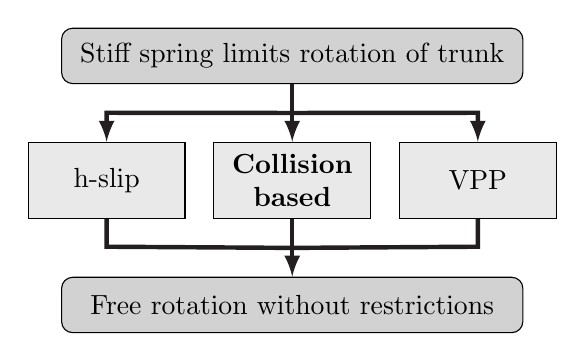
\begin{tikzpicture}[scale = 1, node distance = 4.5em]%
    %
    \tikzstyle{arrow} = [->, -latex, draw, ultra thick, color=TUMBlack]%
    \tikzstyle{bigblock} = [rectangle, draw, fill=TUMBlack!20, text width=16em, text badly centered, rounded corners, minimum height=2em]%
    \tikzstyle{block} = [rectangle, draw, fill=TUMBlack!10, text width=5em, text badly centered, minimum height=2.75em]%
    % 
    \node [bigblock] (start) {Stiff spring limits rotation of trunk};%
    % 
    \node [block, below of = start] (collision-based) {\textbf{Collision based}};%
    \node [block, left = 1em of collision-based] (h-slip) {\acrshort{h-slip}};%
    \node [block, right = 1em of collision-based] (vpp) {VPP};%
    %
    \node [bigblock, below of = collision-based] (end) {Free rotation without restrictions};%
    %
    \coordinate [above = 1.05em of h-slip] (B);%
    \coordinate [above = 1.05em of vpp] (C);%
    \path [arrow] (start) -- (collision-based) node [midway] (A) {};%
    \path [arrow] (A.center) -- (B) -- (h-slip.north);%
    \path [arrow] (A.center) -- (C) -- (vpp.north);%
    %
    \coordinate [below = 1em of h-slip] (D);%
    \coordinate [below = 1em of vpp] (E);%
    \path [arrow] (collision-based) -- (end) node [midway] (F) {};%
    \path [draw, ultra thick, color=TUMBlack] (h-slip.south) -- (D) -- (F.center);%
    \path [draw, ultra thick, color=TUMBlack] (vpp.south) -- (E) -- (F.center);%
\end{tikzpicture}%
%
\end{document}%
%